\section{実験結果と考察}
基準AによるBの校正時のドリフト測定の結果を図\ref{fig:ドリフト1}に示す.変位計Aの変位は負の方向に傾くように変化したが,変位計Bはほとんど変位していなかった.
基準BによるAの校正時のドリフト測定の結果を図\ref{fig:ドリフト2}に示す.変位計Aは変位0.060mm/divでほぼ一定だったが,変位計Bは負の方向に傾くようなグラフとなった.

\begin{figure}[htbp]
    \centering %中央揃え
    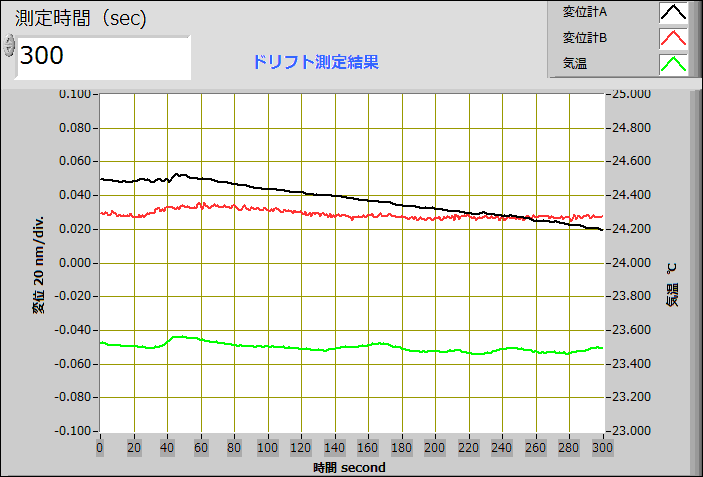
\includegraphics[width=100truemm,clip]{fig/温度ドリフト測定結果(Step1前)_A.png}
    \caption{Temperature drift measurement results(Calibration of B with reference A).}
    \label{fig:ドリフト1}
\end{figure}
\begin{figure}[htbp]
    \centering %中央揃え
    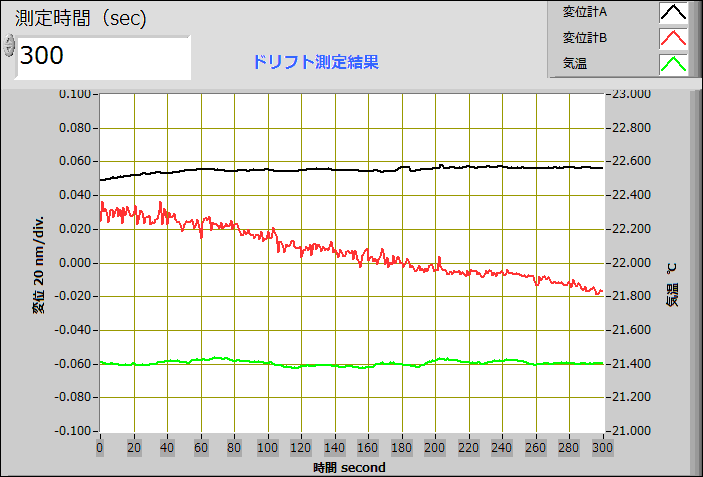
\includegraphics[width=100truemm,clip]{fig/温度ドリフト測定結果(Step2前)_A.png}
    \caption{Temperature drift measurement results(Calibration of A with reference B).}
    \label{fig:ドリフト2}
\end{figure}

図\ref{fig:測定結果}に測定した校正曲線と室温のグラフを示す.
\begin{figure}[htbp]
    \centering %中央揃え
    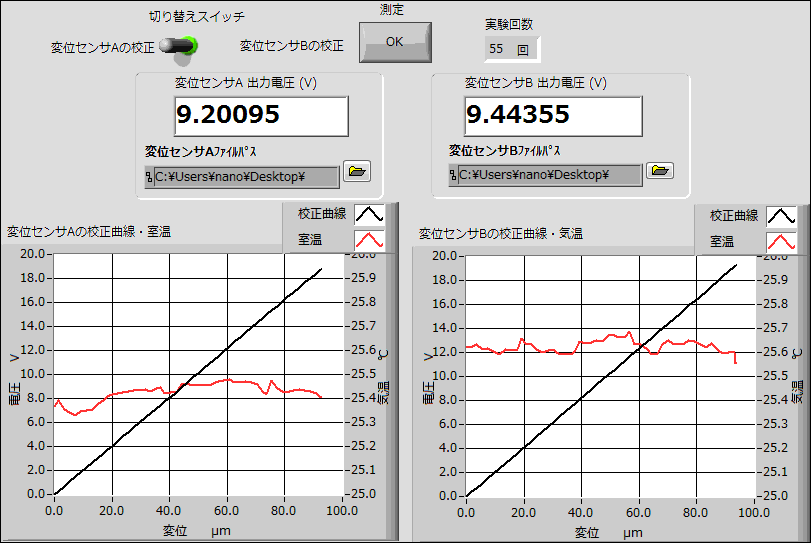
\includegraphics[width=100truemm,clip]{fig/測定結果_D.png}
    \caption{Calibration curve and room temperature measurement results.}
    \label{fig:測定結果}
\end{figure}

図\ref{fig:演算結果}には,演算により得られた校正曲線と線形誤差のグラフを示す.線形誤差はグラフが重なっており,実験で求めた結果と5回目の結果のみが表示されている.このことから誤差が収束しており,得られた校正曲線は有効であると考えられる.図\ref{fig:演算結果}において式(\ref{eq:誤差Ak-1}),(\ref{eq:誤差Bk})はk=12,n=5である.演算5回目の値が真の値に十分近いと考えると,演算5回目の線形誤差の絶対値の平均はおよそ0.1$\mu$mであるから,期待される校正曲線の誤差は以下のように概算できる.
\begin{equation}
    e_{A12} = \frac{e_{A0}}{5^{12}} = \frac{0.1}{5^{12}} \approx 4.1 \times 10^{-10}[\mu m]
\end{equation}

次に再現性について考察する.n=5であるから,20$\mu$mごとに同じような波形が繰り返し現れるはずである.しかし,図\ref{fig:演算結果}において波形にはばらつきが大きく,再現性は低いものと考えられる.再現誤差の原因としては,温度変化によるドリフトや,レバーの変形,振動,回路のノイズ,センサの値が画面上に表示されるまでの遅れ等が考えられる.演算5回目の線形誤差の最大絶対値はおよそ0.2$\mu$mであることを用いて,期待される校正曲線の誤差を以下のように概算した.
\begin{equation}
    e_{A12} = \frac{e_{A0}}{5^{12}} = \frac{0.2}{5^{12}} \approx 8.2 \times 10^{-10}[\mu m]
\end{equation}

\begin{figure}[htbp]
    \centering %中央揃え
    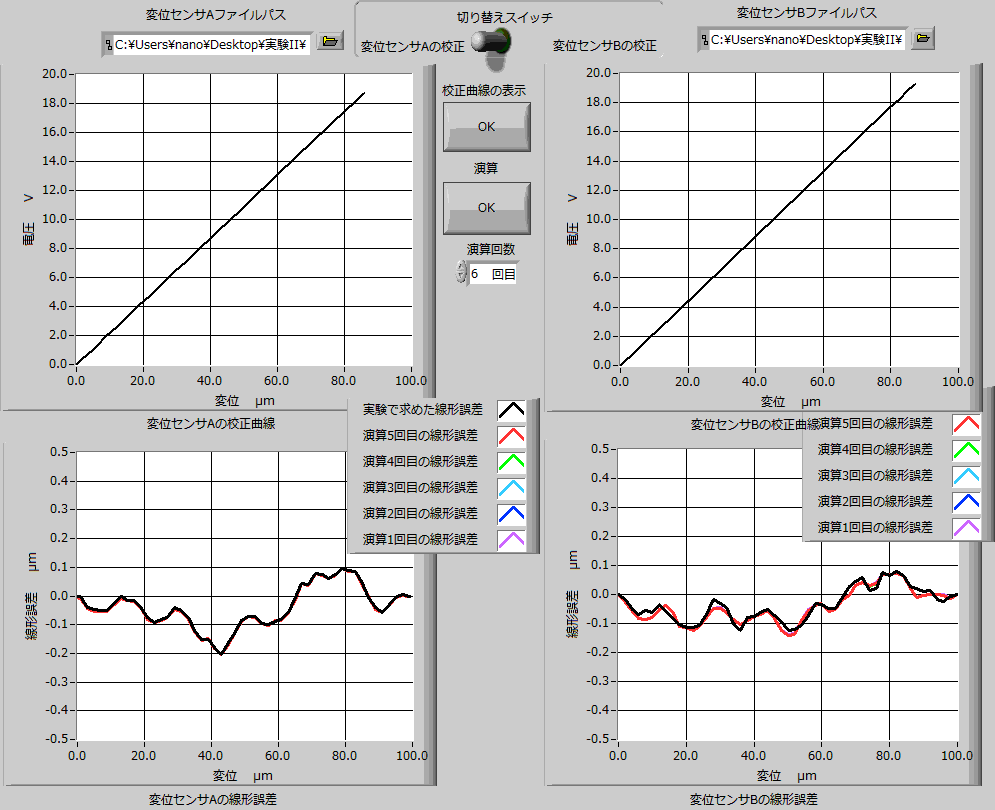
\includegraphics[width=100truemm,clip]{fig/演算結果_A.png}
    \caption{Graphs of calibration curves and their linear errors due to arithmetic operations.}
    \label{fig:演算結果}
\end{figure}

温度の影響について考察する.図\ref{fig:ドリフト1},\ref{fig:ドリフト2}から温度がほぼ一定にもかかわらず,変位計の値が変化しており,最大で0.040$\mu$mの変化がみられる.図\ref{fig:測定結果}では,図\ref{fig:ドリフト1},\ref{fig:ドリフト2}のときよりも大きい温度変化が見られていることから,さらに大きいドリフトが生じさせていることが想定され,校正曲線の再現性・精度に影響を及ぼしていると考えられる.